\documentclass[aspectratio=169, 10pt]{beamer}

% ============================================================
% ชุดสไลด์นำเสนอระดับ Masterclass (16:9 Widescreen Presentation)
% หลักสูตรเกษตรดิจิทัลและปัญญาประดิษฐ์ฝังตัว
% คณะวิทยาศาสตร์และเทคโนโลยี มหาวิทยาลัยราชภัฏรำไพพรรณี
% ============================================================

\usepackage{fontspec}
\usepackage{xcolor}
\usepackage{tikz}
\usetikzlibrary{shapes, arrows.meta, positioning, calc, backgrounds}
\usepackage{amsmath, amssymb}
\usepackage{booktabs}
\usepackage{tabularx}
\usepackage{listings}
\usepackage[many]{tcolorbox}
\usepackage{multicol}

% ตั้งค่าฟอนต์ภาษาไทยสำหรับ Beamer
\usefonttheme{professionalfonts}
\setmainfont{Sarabun}
\setsansfont{Sarabun}
\XeTeXlinebreaklocale "th"
\XeTeXlinebreakskip = 0pt plus 1pt

% นิยามชุดสีทางการ มหาวิทยาลัยราชภัฏรำไพพรรณี
\definecolor{rbruNavy}{RGB}{16, 37, 66}       % สีน้ำเงินเข้มราชภัฏ
\definecolor{rbruGold}{RGB}{212, 160, 23}     % สีทองราชภัฏ
\definecolor{agriForest}{RGB}{34, 112, 62}    % สีเขียวเกษตรอัจฉริยะ
\definecolor{aquaCyan}{RGB}{18, 148, 180}     % สีฟ้าครามวาริชศาสตร์
\definecolor{durianGold}{RGB}{224, 159, 31}   % สีเหลืองทองทุเรียน
\definecolor{slateGrey}{RGB}{85, 100, 115}    % สีเทาสเลท
\definecolor{lightGrey}{RGB}{246, 248, 251}   % สีเทาพื้นหลัง
\definecolor{darkText}{RGB}{25, 30, 40}       % สีข้อความหลัก
\definecolor{cardBorder}{RGB}{218, 225, 233}  % สีกรอบการ์ด

% กำหนดสไตล์ Beamer
\setbeamercolor{background canvas}{bg=white}
\setbeamercolor{normal text}{fg=darkText}
\setbeamercolor{frametitle}{bg=rbruNavy, fg=white}
\setbeamercolor{title}{fg=white}
\setbeamercolor{item}{fg=rbruNavy}
\setbeamerfont{frametitle}{size=\large, series=\bfseries}

% ซ่อนปุ่มนำทางเริ่มต้นของ Beamer
\setbeamertemplate{navigation symbols}{}

% ออกแบบแถบหัวสไลด์ (Header)
\setbeamertemplate{frametitle}{%
    \nointerlineskip%
    \begin{beamercolorbox}[wd=\paperwidth, ht=1.1cm, dp=0.3cm, leftskip=0.8cm, rightskip=0.8cm]{frametitle}%
        
\begin{tikzpicture}[remember picture, overlay]
            \fill[color=rbruGold] (0, -0.32cm) rectangle (\paperwidth, -0.36cm);
        \end{tikzpicture}%
        \vspace{-0.1cm}%
        \insertframetitle \hfill {\small\normalfont\color{rbruGold!90} SCIRBRU AIoT 2570}%
    \end{beamercolorbox}%
}

% ออกแบบแถบท้ายสไลด์ (Footer)
\setbeamertemplate{footline}{%
    \leavevmode%
    \hbox{%
        \begin{beamercolorbox}[wd=0.55\paperwidth, ht=0.4cm, dp=0.15cm, leftskip=0.8cm]{normal text}%
            {\fontsize{7.5}{9}\selectfont\color{slateGrey} หลักสูตรเกษตรดิจิทัลและปัญญาประดิษฐ์ฝังตัว ภาคตะวันออก}%
        \end{beamercolorbox}%
        \begin{beamercolorbox}[wd=0.45\paperwidth, ht=0.4cm, dp=0.15cm, rightskip=0.8cm]{normal text}%
            \raggedleft{\fontsize{7.5}{9}\selectfont\color{slateGrey} ผศ.ดร.ชีวะ ทัศนา และคณะ \quad \textbar \quad \bfseries\color{rbruNavy}\insertframenumber{} / \inserttotalframenumber}%
        \end{beamercolorbox}%
    }%
}

% กล่องข้อมูลสวยงามสไตล์ Modern Academic Card
\newtcolorbox{mastercard}[2][]{
    enhanced,
    colback=white,
    colframe=rbruNavy,
    coltitle=white,
    colbacktitle=rbruNavy,
    title={\bfseries #2},
    fonttitle=\fontsize{9.5}{11}\selectfont\bfseries,
    fontupper=\fontsize{8.5}{11.5}\selectfont,
    arc=3pt,
    boxrule=1pt,
    titlerule=0pt,
    left=6pt, right=6pt, top=6pt, bottom=6pt,
    drop shadow=cardBorder!80,
    #1
}

\newtcolorbox{goldcard}[2][]{
    enhanced,
    colback=lightGrey,
    colframe=durianGold!90!black,
    coltitle=white,
    colbacktitle=durianGold!90!black,
    title={\bfseries #2},
    fonttitle=\fontsize{9.5}{11}\selectfont\bfseries,
    fontupper=\fontsize{8.5}{11.5}\selectfont,
    arc=3pt,
    boxrule=1pt,
    left=6pt, right=6pt, top=6pt, bottom=6pt,
    #1
}

\newtcolorbox{aquacard}[2][]{
    enhanced,
    colback=aquaCyan!5!white,
    colframe=aquaCyan!90!black,
    coltitle=white,
    colbacktitle=aquaCyan!90!black,
    title={\bfseries #2},
    fonttitle=\fontsize{9.5}{11}\selectfont\bfseries,
    fontupper=\fontsize{8.5}{11.5}\selectfont,
    arc=3pt,
    boxrule=1pt,
    left=6pt, right=6pt, top=6pt, bottom=6pt,
    #1
}

\newtcolorbox{notecard}[1][]{
    enhanced,
    colback=lightGrey,
    colframe=cardBorder,
    arc=3pt,
    boxrule=0.6pt,
    left=6pt, right=6pt, top=3pt, bottom=3pt,
    fontupper=\scriptsize,
    #1
}

\begin{document}

% ============================================================
% SLIDE 1: ปกหน้านำเสนอระดับ Masterclass (Title Slide)
% ============================================================
{
\setbeamertemplate{footline}{}
\begin{frame}[plain]
\begin{tikzpicture}[remember picture, overlay]
    % พื้นหลังไล่ระดับสีน้ำเงินเข้ม
    \fill[left color=rbruNavy!98!black, right color=rbruNavy!88!agriForest] 
        (current page.south west) rectangle (current page.north east);
    
    % แถบขลิบทองราชภัฏ
    \fill[color=rbruGold] 
        ([xshift=0.7cm]current page.south west) rectangle ([xshift=0.82cm]current page.north west);

    % ข้อมูลและเนื้อหาด้านซ้ายทั้งหมดในบล็อกเดียว
    \node[anchor=north west, text width=7.6cm] at ([xshift=1.1cm, yshift=-0.6cm]current page.north west) {
        {\fontsize{10}{12.5}\selectfont\bfseries\color{rbruGold} คณะวิทยาศาสตร์และเทคโนโลยี มหาวิทยาลัยราชภัฏรำไพพรรณี\par}
        \vspace{2pt}
        {\fontsize{7}{9}\selectfont\color{white!80} โครงการพัฒนาทักษะวิชาชีพชั้นสูงเพื่อการขับเคลื่อนเศรษฐกิจฐานนวัตกรรม (AIoT 2570)\par}
        \vspace{5pt}
        {\color{rbruGold}\rule{6.8cm}{1.2pt}\par}
        \vspace{6pt}
        {\fontsize{17.5}{21}\selectfont\bfseries\color{white} หลักสูตรเกษตรดิจิทัล\par}
        \vspace{2pt}
        {\fontsize{16.5}{20}\selectfont\bfseries\color{white} และปัญญาประดิษฐ์ฝังตัว\par}
        \vspace{4pt}
        {\fontsize{9.5}{12.5}\selectfont\bfseries\color{durianGold} สวนผลไม้มูลค่าสูงและการเพาะเลี้ยงสัตว์น้ำชายฝั่ง ภาคตะวันออก\par}
        \vspace{3pt}
        {\fontsize{6.5}{8.5}\selectfont\color{white!70} Digital Agriculture and Embedded Artificial Intelligence Curriculum\par}
        \vspace{6pt}
        {\color{rbruGold}\rule{6.8cm}{0.8pt}\par}
        \vspace{5pt}
        {\fontsize{8.5}{10.5}\selectfont\bfseries\color{white} ผู้ช่วยศาสตราจารย์ ดร.ชีวะ ทัศนา (ผู้นิพนธ์หลักและบรรณาธิการ)\par}
        \vspace{1pt}
        {\fontsize{7}{9}\selectfont\color{white!80} ร่วมกับคณะวิทยากรผู้เชี่ยวชาญ คณะวิทยาศาสตร์และเทคโนโลยี 8 ท่าน\par}
        \vspace{3pt}
        {\fontsize{7}{9}\selectfont\color{rbruGold} สำนักพิมพ์มหาวิทยาลัยราชภัฏรำไพพรรณี \quad \textbar \quad พ.ศ. 2570\par}
    };

    % กรอบภาพศิลป์ปก Masterclass ด้านขวา
    \node[anchor=east, draw=rbruGold, line width=1.5pt, rounded corners=5pt, inner sep=0pt, fill=black] 
        at ([xshift=-0.5cm, yshift=0cm]current page.east) {
        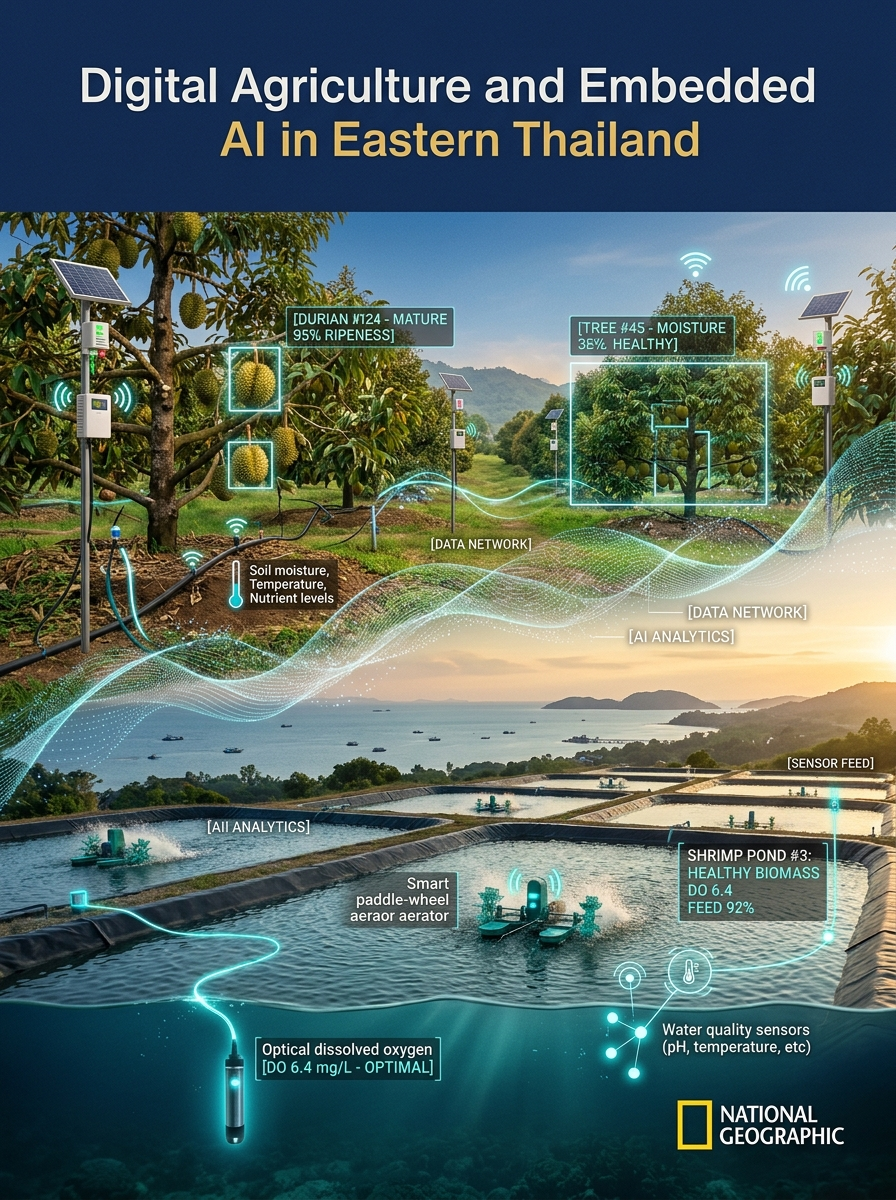
\includegraphics[width=6.0cm, height=7.2cm, keepaspectratio=false]{figures/cover_artwork.jpg}
    };
\end{tikzpicture}
\end{frame}
}

% ============================================================
% SLIDE 2: วัตถุประสงค์และบริบทการพัฒนาหลักสูตร
% ============================================================
\begin{frame}{วัตถุประสงค์และบริบทการพัฒนาหลักสูตร}
\begin{columns}[T]
    \begin{column}{0.48\textwidth}
        \begin{mastercard}{ความท้าทายเชิงโครงสร้างของภาคตะวันออก}
            \begin{itemize}
                \item \textbf{ศูนย์กลางเศรษฐกิจเกษตรมูลค่าสูง} แหล่งผลิตทุเรียน มังคุด และกุ้งขาวแวนนาไมส่งออกหลักของประเทศ
                \item \textbf{สภาพภูมิอากาศผันผวน} ฝนทิ้งช่วง ภัยแล้ง และน้ำเค็มรุกแปลงสวนผลไม้
                \item \textbf{ต้นทุนพลังงานและแรงงานสูง} เครื่องตีน้ำบ่อกุ้งกินไฟสูง ขาดแคลนแรงงานผู้เชี่ยวชาญ
                \item \textbf{ปัญหาคุณภาพผลผลิต} การตัดทุเรียนอ่อน และโรคระบาดในฟาร์มเพาะเลี้ยงสัตว์น้ำ
            \end{itemize}
        \end{mastercard}
    \end{column}
    \begin{column}{0.48\textwidth}
        \begin{goldcard}{เป้าหมายและผลลัพธ์การเรียนรู้ (OBE)}
            \begin{itemize}
                \item \textbf{บูรณาการศาสตร์ข้ามสาขา} ฟิสิกส์เกษตร เคมีวิเคราะห์ สมองกลฝังตัว และ Edge AI
                \item \textbf{ปฏิบัติการหน้างานจริง (Active Learning)} 120 ชั่วโมงการเรียนรู้ (บรรยาย 45 ชม. ปฏิบัติการ 75 ชม.)
                \item \textbf{สร้างนวัตกรแก้ไขปัญหาได้ตรงจุด} ประหยัดพลังงาน ยกระดับมาตรฐานการส่งออก
                \item \textbf{โครงงานบูรณาการภาคสนาม 50\%} พัฒนาต้นแบบนวัตกรรมพร้อมใช้งานในแปลงจริง
            \end{itemize}
        \end{goldcard}
    \end{column}
\end{columns}
\end{frame}

% ============================================================
% SLIDE 3: สถาปัตยกรรมระบบรวม Eastern Agri-Aqua AIoT
% ============================================================
\begin{frame}{สถาปัตยกรรมระบบนิเวศ Eastern Agri-Aqua AIoT}
\centering
\begin{tikzpicture}[scale=0.85, every node/.style={transform shape}]
    % Layer 1: Perception
    \node[draw=agriForest, fill=agriForest!10, rounded corners=4pt, text width=3.4cm, align=center, minimum height=1.3cm] (sens) at (0, 3.2) {
        \textbf{\color{agriForest} 1. ตรวจวัดทางฟิสิกส์}\\[2pt]
        {\scriptsize โพรบดิน 7-in-1, NPK, สภาพอากาศ, Optical DO, ความเค็ม}
    };
    
    % Layer 2: Edge Computing
    \node[draw=rbruNavy, fill=rbruNavy!10, rounded corners=4pt, text width=3.4cm, align=center, minimum height=1.3cm] (edge) at (4.5, 3.2) {
        \textbf{\color{rbruNavy} 2. ประมวลผลที่ขอบ}\\[2pt]
        {\scriptsize ESP32-S3 Dual-Core, FreeRTOS, TinyML, OpenCV, FFT}
    };
    
    % Layer 3: High Power Actuation
    \node[draw=durianGold!90!black, fill=durianGold!10, rounded corners=4pt, text width=3.4cm, align=center, minimum height=1.3cm] (act) at (9.0, 3.2) {
        \textbf{\color{durianGold!90!black} 3. ควบคุมโหลดกำลังสูง}\\[2pt]
        {\scriptsize วาล์ว 24VAC ป้องกัน Water Hammer, VFD ขับเครื่องตีน้ำ}
    };
    
    % Layer 4: Telemetry
    \node[draw=aquaCyan!90!black, fill=aquaCyan!10, rounded corners=4pt, text width=5.5cm, align=center, minimum height=1.1cm] (comm) at (2.2, 1.2) {
        \textbf{\color{aquaCyan!90!black} 4. เครือข่ายไร้สายระยะไกล}\\[2pt]
        {\scriptsize ESP-NOW Bridge $\leftrightarrow$ LoRaWAN AS923 (Duty Cycle $\le 1\%$)}
    };
    
    % Layer 5: Cloud & Decision
    \node[draw=rbruGold!90!black, fill=rbruGold!10, rounded corners=4pt, text width=5.5cm, align=center, minimum height=1.1cm] (cloud) at (8.0, 1.2) {
        \textbf{\color{rbruGold!90!black} 5. คลาวด์และแดชบอร์ดตัดสินใจ}\\[2pt]
        {\scriptsize MQTT Broker, Time-Series DB, Closed-Loop Control, LINE Alert}
    };

    % Arrows
    \draw[-{Stealth[length=5pt]}, thick, color=rbruNavy] (sens) -- (edge);
    \draw[-{Stealth[length=5pt]}, thick, color=rbruNavy] (edge) -- (act);
    \draw[-{Stealth[length=5pt]}, thick, color=aquaCyan] (edge.south) -- ++(0, -0.4) -| (comm.north);
    \draw[-{Stealth[length=5pt]}, thick, color=aquaCyan] (comm) -- (cloud);
    \draw[-{Stealth[length=5pt]}, dashed, thick, color=agriForest] (cloud.north) -- ++(0, 0.4) -| (act.south);
\end{tikzpicture}

\vspace{0.1cm}
\begin{notecard}
    {\bfseries\color{rbruNavy} จุดเด่นทางวิศวกรรม} ทำงานแบบ Two-Stage Decoupling คือ ควบคุมโหลดวิกฤตได้อัตโนมัติหน้างานแม้เครือข่ายอินเทอร์เน็ตขัดข้อง
\end{notecard}
\end{frame}

% ============================================================
% SLIDE 4: ฟิสิกส์เกษตรดิจิทัลและสภาพแวดล้อมจุลภาค
% ============================================================
\begin{frame}{บทที่ 1: วิศวกรรมฟิสิกส์เกษตรและสภาพแวดล้อมจุลภาค}
\begin{columns}[T]
    \begin{column}{0.48\textwidth}
        \begin{mastercard}{สมการพันธุกรรมและสิ่งแวดล้อม}
            \begin{equation*}
                P = G + E + (G \times E)
            \end{equation*}
            \begin{itemize}
                \item $P$ ผลผลิตที่แสดงออกจริง (Phenotype)
                \item $G$ ศักยภาพสูงสุดทางพันธุกรรม (Genotype)
                \item $E$ สิ่งแวดล้อม ดิน น้ำ แสง อุณหภูมิ
                \item \textbf{$G \times E$ ปฏิสัมพันธ์ระหว่างพันธุ์กับสิ่งแวดล้อม} หัวใจของระบบ AIoT ในการควบคุมสิ่งแวดล้อมให้เข้ากับสายพันธุ์พืช
            \end{itemize}
        \end{mastercard}
    \end{column}
    \begin{column}{0.48\textwidth}
        \begin{goldcard}{แรงดึงระเหยน้ำของอากาศ (VPD)}
            \begin{equation*}
                \text{VPD} = e_s(T) \times \left(1 - \frac{\text{RH}}{100}\right)
            \end{equation*}
            \begin{itemize}
                \item ขับเคลื่อนการคายน้ำและการดูดซึมแคลเซียมทางราก
                \item \textbf{VPD เหมาะสม} $0.8 - 1.2\text{ kPa}$ พืชเปิดปากใบสมบูรณ์
                \item \textbf{VPD ต่ำเกินไป} อับชื้น เสี่ยงโรคราใบติด
                \item \textbf{VPD สูงเกินไป} อากาศแห้ง พืชปิดปากใบเพื่อเอาชีวิตรอด
            \end{itemize}
        \end{goldcard}
    \end{column}
\end{columns}
\end{frame}

% ============================================================
% SLIDE 5: เทคโนโลยีเซนเซอร์ตรวจวัดคุณภาพดินและน้ำ
% ============================================================
\begin{frame}{เทคโนโลยีเซนเซอร์ตรวจวัดดิน สภาพอากาศ และน้ำชายฝั่ง}
\begin{columns}[T]
    \begin{column}{0.48\textwidth}
        \begin{mastercard}{โพรบวัดดินอเนกประสงค์ 7-in-1 RS-485}
            \begin{itemize}
                \item ตรวจวัดค่าความชื้น อุณหภูมิ การนำไฟฟ้า (EC) กรดด่าง (pH) และปริมาณธาตุอาหาร N-P-K
                \item \textbf{สมการเนิร์นสต์ (Nernst Equation)}
                \begin{equation*}
                    E = E^0 - \frac{2.303RT}{F}\text{pH}
                \end{equation*}
                ความชันลดลง $59.16\text{ mV/pH}$ ที่อุณหภูมิ $25^\circ\text{C}$
                \item สื่อสารผ่านโพรโทคอล Modbus RTU ความเร็ว $9600\text{ bps}$ ตรวจสอบความถูกต้องด้วย CRC-16
            \end{itemize}
        \end{mastercard}
    \end{column}
    \begin{column}{0.48\textwidth}
        \begin{aquacard}{โพรบวัดออกซิเจนละลายเชิงแสง (Optical DO)}
            \begin{itemize}
                \item ใช้หลักการลดทอนความสว่างของสารเรืองแสง (Fluorescence Quenching) เมื่อสัมผัสโมเลกุลออกซิเจน
                \item \textbf{สมการสเตอร์น-โวลเมอร์ (Stern-Volmer)}
                \begin{equation*}
                    \frac{\tau_0}{\tau} = 1 + K_{SV}[\text{DO}]
                \end{equation*}
                \item \textbf{ข้อได้เปรียบเหนือโพรบกัลวานิก} ไม่บริโภคออกซิเจน ไม่ต้องมีกระแสน้ำไหลผ่าน และบำรุงรักษาง่าย
            \end{itemize}
        \end{aquacard}
    \end{column}
\end{columns}
\end{frame}

% ============================================================
% SLIDE 6: สถาปัตยกรรมสมองกลฝังตัว ESP32-S3 Dual-Core
% ============================================================
\begin{frame}{บทที่ 2: สถาปัตยกรรมสมองกลฝังตัวและการประมวลผลเวลาจริง}
\begin{columns}[T]
    \begin{column}{0.48\textwidth}
        \begin{mastercard}{สถาปัตยกรรม ESP32-S3 Dual-Core}
            \begin{itemize}
                \item \textbf{Core 0 (Communication Core)} จัดการ WiFi, ESP-NOW, LoRaWAN Stack และ Modbus RTU Master
                \item \textbf{Core 1 (Real-Time Control Core)} สุ่มอ่านสัญญาณ ADC ขับสัญญาณ PWM และคำนวณอัลกอริทึม
                \item \textbf{หน่วยความจำเสริม} 8MB Octal PSRAM รองรับการพักเฟรมภาพสำหรับโมเดลคอมพิวเตอร์วิทัศน์
                \item \textbf{Hardware Vector Instructions} เร่งความเร็วการคำนวณพีชคณิตเชิงเส้นและโครงข่ายประสาท
            \end{itemize}
        \end{mastercard}
    \end{column}
    \begin{column}{0.48\textwidth}
        \begin{goldcard}{การแบ่งงานด้วยระบบปฏิบัติการเวลาจริง (FreeRTOS)}
            \begin{itemize}
                \item \textbf{Sensor Acquisition Task} ความสำคัญปานกลาง อ่านค่าเซนเซอร์ทุก 5 วินาที
                \item \textbf{Emergency Shutdown Task} ความสำคัญสูงสุด ตรวจจับกระแสเกินและแรงดันตกใน 50 มิลลิวินาที
                \item \textbf{Actuation Control Task} คำนวณ Closed-Loop และสั่งงานรีเลย์หรือวาล์วไฟฟ้า
                \item \textbf{Telemetry Transmission Task} นำข้อมูลเข้า FreeRTOS Queue เพื่อแพ็กส่งขึ้นคลาวด์
            \end{itemize}
        \end{goldcard}
    \end{column}
\end{columns}
\end{frame}

% ============================================================
% SLIDE 7: การควบคุมโหลดกำลังสูงและการป้องกัน Water Hammer
% ============================================================
\begin{frame}{การควบคุมโหลดกำลังสูงและการป้องกันปรากฏการณ์ค้อนน้ำ}
\begin{columns}[T]
    \begin{column}{0.48\textwidth}
        \begin{mastercard}{โซเลนอยด์วาล์ว 24VAC ซอฟต์โคลส}
            \begin{itemize}
                \item ขับด้วยกระแสสลับ 24VAC ปลอดภัยต่อเกษตรกรในพื้นที่เปียกชื้น
                \item ขับผ่านชิป Solid State Relay หรือ Triac เบอร์ BTA16 พร้อมออปโต้คัปเปลอร์ MOC3041 (Zero-Cross)
                \item \textbf{ป้องกันปรากฏการณ์ค้อนน้ำ (Water Hammer)} ด้วยกลไก Pilot-operated Diaphragm ปิดวาล์วนุ่มนวลภายในเวลา $1.5 - 3.0$ วินาที
                \item ป้องกันคลื่นความดันกระแทกสูงเกิน $10\text{ bar}$ ซึ่งทำให้ท่อ PVC แตกหัก
            \end{itemize}
        \end{mastercard}
    \end{column}
    \begin{column}{0.48\textwidth}
        \begin{goldcard}{การควบคุมอินเวอร์เตอร์ VFD ผ่าน RS-485}
            \begin{itemize}
                \item สื่อสารกับอินเวอร์เตอร์ VFD ขับมอเตอร์เหนี่ยวนำ 3 เฟส $380\text{V}$ หรือ 1 เฟส $220\text{V}$
                \item เขียนรีจิสเตอร์ความถี่ผ่าน Modbus Function Code 06 (Write Single Register)
                \item สั่งเร่งและลดความเร็วตามแนวเส้นโค้ง (S-Curve Acceleration/Deceleration)
                \item ลดกระแสกระชากขณะสตาร์ทมอเตอร์จาก 6 เท่าเหลือเท่ากับพิกัดปกติ
            \end{itemize}
        \end{goldcard}
    \end{column}
\end{columns}
\end{frame}

% ============================================================
% SLIDE 8: ชลศาสตร์สวนผลไม้และการใช้น้ำของทุเรียน
% ============================================================
\begin{frame}{บทที่ 3: ชลศาสตร์สวนผลไม้และการคำนวณการใช้น้ำของทุเรียน}
\begin{columns}[T]
    \begin{column}{0.48\textwidth}
        \begin{mastercard}{การคำนวณการคายระเหยน้ำจริง ($ET_c$)}
            \begin{equation*}
                ET_c = K_c \times ET_0
            \end{equation*}
            \begin{itemize}
                \item $ET_0$ การคายระเหยน้ำอ้างอิงจากรังสีดวงอาทิตย์ อุณหภูมิ และลม
                \item $K_c$ สัมประสิทธิ์พืชตามระยะพัฒนาการของทุเรียน
                \item \textbf{ระยะกระตุ้นตาดอก} ลดน้ำ งดน้ำ $K_c \approx 0.5$
                \item \textbf{ระยะดอกบาน} รดน้ำร้อยละ 30-40 ป้องกันดอกร่วง
                \item \textbf{ระยะพัฒนาการผล} ให้น้ำเต็มที่ $K_c \approx 0.95 - 1.05$
                \item \textbf{ระยะก่อนเก็บเกี่ยว} ลดน้ำ 10 วัน เพิ่มความหวาน
            \end{itemize}
        \end{mastercard}
    \end{column}
    \begin{column}{0.48\textwidth}
        \begin{goldcard}{อัตราการไหลรวมของระบบชลศาสตร์ ($Q$)}
            \begin{equation*}
                Q = \frac{A \times ET_c}{T \times \text{Eff}}
            \end{equation*}
            \begin{itemize}
                \item $A$ พื้นที่เพาะปลูกหรือทรงพุ่ม (ตารางเมตร)
                \item $T$ ระยะเวลาการให้น้ำต่อวัน (ชั่วโมง)
                \item $\text{Eff}$ ประสิทธิภาพหัวจ่ายน้ำ มินิสปริงเกลอร์ $85\%$ น้ำหยด $90\%$
                \item กำหนดขนาดหัวมินิสปริงเกลอร์ 2-3 หัวต่อต้นเพื่อครอบคลุมรัศมีรากหากิน
            \end{itemize}
        \end{goldcard}
    \end{column}
\end{columns}
\end{frame}

% ============================================================
% SLIDE 9: การคำนวณแรงดันสูญเสียในท่อและเฮดปั๊มน้ำ
% ============================================================
\begin{frame}{การคำนวณแรงดันสูญเสียในท่อและเฮดรวมของปั๊มน้ำ}
\begin{columns}[T]
    \begin{column}{0.48\textwidth}
        \begin{mastercard}{สมการการสูญเสียแรงดัน Hazen-Williams}
            \begin{equation*}
                h_f = 10.67 \times L \times Q^{1.852} \times C^{-1.852} \times D^{-4.87}
            \end{equation*}
            \begin{itemize}
                \item $C$ สัมประสิทธิ์ความขรุขระของท่อ ท่อ PVC และ PE $C = 140 - 150$
                \item \textbf{เกณฑ์ความเร็วการไหลที่เหมาะสม}
                \begin{itemize}
                    \item ท่อเมนหลัก $1.5 - 2.0\text{ m/s}$
                    \item ท่อเมนย่อย $1.2 - 1.8\text{ m/s}$
                    \item ท่อแขนง PE $0.6 - 1.2\text{ m/s}$
                \end{itemize}
                \item ป้องกันท่อเล็กเกินไปซึ่งทำให้เกิดความสูญเสีย $h_f \propto v^2$ สูง
            \end{itemize}
        \end{mastercard}
    \end{column}
    \begin{column}{0.48\textwidth}
        \begin{goldcard}{เฮดรวมและการเลือกกำลังปั๊มน้ำ}
            \begin{equation*}
                \text{TDH} = H_{\text{static}} + h_f + h_m + H_{\text{operating}}
            \end{equation*}
            \begin{itemize}
                \item $H_{\text{static}}$ ความต่างระดับแนวดิ่งจากผิวน้ำถึงจุดสูงสุด
                \item $h_m$ Minor loss ในข้องอ วาล์ว กรองน้ำ ($20\%$ ของ $h_f$)
                \item $H_{\text{operating}}$ แรงดันหัวมินิสปริงเกลอร์ ($15 - 20\text{ m}$)
                \item \textbf{กำลังมอเตอร์ปั๊มน้ำ (แรงม้า)}
                \begin{equation*}
                    HP = \frac{\rho \cdot g \cdot Q \cdot \text{TDH}}{746 \times \eta}
                \end{equation*}
            \end{itemize}
        \end{goldcard}
    \end{column}
\end{columns}
\end{frame}

% ============================================================
% SLIDE 10: คอมพิวเตอร์วิทัศน์ตัดสีร่องหนามทุเรียน (HSV)
% ============================================================
\begin{frame}{บทที่ 4: การประเมินความสุกแก่ทุเรียนด้วยคอมพิวเตอร์วิทัศน์}
\begin{columns}[T]
    \begin{column}{0.48\textwidth}
        \begin{mastercard}{ทำไมระบบสี RGB จึงล้มเหลวในแปลงจริง?}
            \begin{itemize}
                \item ระบบสี RGB รวมข้อมูลความสว่างและเฉดสีไว้ในช่องสัญญาณเดียวกัน
                \item เมื่อผลทุเรียนอยู่ใต้เงาใบไม้ ค่าพิกเซล R, G, B จะตกลงพร้อมกัน คอมพิวเตอร์จึงเข้าใจผิดว่าเป็นรอยโรคหรือผลเน่า
                \item \textbf{ทางออกด้วยปริภูมิสี HSV}
                \begin{itemize}
                    \item $H$ (Hue) เฉดสีแท้จริง ไม่ขึ้นกับแสงเงา
                    \item $S$ (Saturation) ความสดของสี
                    \item $V$ (Value) ระดับความสว่าง
                \end{itemize}
            \end{itemize}
        \end{mastercard}
    \end{column}
    \begin{column}{0.48\textwidth}
        \begin{goldcard}{การตัดแถบสีร่องหนามทุเรียน}
            \begin{itemize}
                \item ทุเรียนแก่จัด ร่องระหว่างหนามจะเปลี่ยนจากเขียวสดเป็นสีน้ำตาลอมเหลือง
                \item กำหนดค่าช่วงสีสุกแก่ในระบบ OpenCV
                \begin{itemize}
                    \item สีร่องหนามแก่ $H \in [18, 35], S \in [50, 255]$
                    \item สีหนามเขียวดิบ $H \in [36, 75], S \in [60, 255]$
                \end{itemize}
                \item คำนวณสัดส่วนพิกเซลสีน้ำตาลร่องหนามต่อพื้นที่ผิวทั้งหมด
                \item เกณฑ์ความสุกแก่มากกว่าร้อยละ 85 ให้ค่าสัดส่วนร่องหนามเกินร้อยละ 65
            \end{itemize}
        \end{goldcard}
    \end{column}
\end{columns}
\end{frame}

% ============================================================
% SLIDE 11: สวนศาสตร์การเคาะเสียงจำแนกความสุกทุเรียน (FFT)
% ============================================================
\begin{frame}{สวนศาสตร์การเคาะเสียงและการแปลงฟูเรียร์แบบเร็ว (FFT)}
\begin{columns}[T]
    \begin{column}{0.48\textwidth}
        \begin{mastercard}{พลวัตการเปลี่ยนแปลงเนื้อทุเรียนเมื่อสุก}
            \begin{itemize}
                \item ทุเรียนดิบ เนื้อเยื่อติดแน่นกับเปลือกด้านใน โครงสร้างแข็งเกร็ง
                \item ทุเรียนสุก เนื้อยุบตัวลงเกิดโพรงอากาศหลวมระหว่างเนื้อกับเปลือก
                \item \textbf{ความแตกต่างของคลื่นเสียง}
                \begin{itemize}
                    \item ทุเรียนดิบ เสียงเคาะแน่นทึบ ความถี่เรโซแนนซ์สูง ($> 650\text{ Hz}$)
                    \item ทุเรียนสุก เสียงเคาะโปร่งหลวม ความถี่ลดต่ำลง ($280 - 450\text{ Hz}$)
                \end{itemize}
            \end{itemize}
        \end{mastercard}
    \end{column}
    \begin{column}{0.48\textwidth}
        \begin{goldcard}{การแปลงสัญญาณ Fast Fourier Transform (FFT)}
            \begin{equation*}
                X(k) = \sum_{n=0}^{N-1} x(n) \cdot e^{-i 2\pi k n / N}
            \end{equation*}
            \begin{itemize}
                \item แปลงสัญญาณเสียงเคาะจากโดเมนเวลาสู่โดเมนความถี่
                \item สกัดตำแหน่งยอดคลื่นสูงสุด (Resonant Peak Frequency)
                \item สหสัมพันธ์เชิงเส้นสูงระหว่างความถี่หลักกับร้อยละเนื้อแห้ง
                \item บูรณาการเป็นเครื่องเคาะทดสอบแบบพกพาไมโครคอนโทรลเลอร์
            \end{itemize}
        \end{goldcard}
    \end{column}
\end{columns}
\end{frame}

% ============================================================
% SLIDE 12: การตรวจจับโรคผลเน่า Phytophthora palmivora
% ============================================================
\begin{frame}{บทที่ 5: การตรวจจับโรคผลเน่าและรากเน่าโคนเน่าทุเรียน}
\begin{columns}[T]
    \begin{column}{0.48\textwidth}
        \begin{mastercard}{เชื้อรา Phytophthora palmivora บนผลทุเรียน}
            \begin{itemize}
                \item เป็นเชื้อราสาเหตุหลักของโรคผลเน่าและรากเน่าโคนเน่า
                \item รอยโรคบนเปลือกมีลักษณะเป็นจุดสีน้ำตาลไหม้ฉ่ำน้ำ ขอบแผลไม่เรียบ
                \item เมื่ออยู่ในตู้คอนเทนเนอร์ขนส่งทางเรือ ความชื้นสูงจะเร่งให้สปอร์ลุกลาม เสียหายทั้งตู้สินค้า
                \item การคัดกรองรอยโรคระยะเริ่มแรกบนสายพานจึงเป็นหัวใจสำคัญอย่างยิ่ง
            \end{itemize}
        \end{mastercard}
    \end{column}
    \begin{column}{0.48\textwidth}
        \begin{goldcard}{กระบวนการเตรียมดาต้าเซ็ตผ่าน Roboflow}
            \begin{itemize}
                \item วาดกรอบสี่เหลี่ยม (Bounding Box) แยก 4 กลุ่ม
                \begin{itemize}
                    \item \texttt{grade\_a} ทรงกลมพูเต็ม ปราศจากแผล
                    \item \texttt{grade\_b} ผลโค้งงอเล็กน้อย ผิวสะอาด
                    \item \texttt{cull} ตกเกรด ทรงบิดเบี้ยว หนามหัก
                    \item \texttt{phytophthora} ตรวจพบรอยโรคผลเน่า
                \end{itemize}
                \item ทำ Data Augmentation พลิกภาพ ปรับแสง เติมสัญญาณรบกวน ทวีคูณข้อมูล 3 เท่า
            \end{itemize}
        \end{goldcard}
    \end{column}
\end{columns}
\end{frame}

% ============================================================
% SLIDE 13: ระบบคัดเกรดผลไม้บนสายพานด้วย YOLOv8/v11
% ============================================================
\begin{frame}{ระบบคัดเกรดผลไม้อัตโนมัติบนสายพานลำเลียง}
\begin{columns}[T]
    \begin{column}{0.48\textwidth}
        \begin{mastercard}{สถาปัตยกรรมโมเดลตรวจจับวัตถุ YOLO}
            \begin{itemize}
                \item ใช้โมเดล YOLOv8n หรือ YOLOv11n ขนาดกะทัดรัด
                \item ตรวจจับและระบุพิกัด $(x, y, w, h)$ พร้อมเปอร์เซ็นต์ความเชื่อมั่น
                \item รันบนคอมพิวเตอร์บอร์ดเดี่ยว (Edge Device) ได้ความเร็วมากกว่า 35 เฟรมต่อวินาที
                \item ความแม่นยำเฉลี่ย mAP@0.5 สูงกว่าร้อยละ 94.2
            \end{itemize}
        \end{mastercard}
    \end{column}
    \begin{column}{0.48\textwidth}
        \begin{goldcard}{การซิงก์ตำแหน่งด้วย Rotary Encoder}
            \begin{itemize}
                \item ติดตั้งโรตารีเอนโค้ดเดอร์วัดความเร็วเชิงเส้นของสายพาน
                \item เมื่อ AI ตรวจพบผลไม้ตกเกรดหรือผลเป็นโรค ระบบจะคำนวณตำแหน่งและหน่วงเวลา
                \begin{equation*}
                    \Delta t = \frac{L_{\text{camera}\to\text{ejector}}}{v_{\text{belt}}}
                \end{equation*}
                \item สั่งหัวฉีดลมหรือแขนกลผลักผลไม้ออกจากสายพานแม่นยำ
            \end{itemize}
        \end{goldcard}
    \end{column}
\end{columns}
\end{frame}

% ============================================================
% SLIDE 14: อุณหพลศาสตร์ออกซิเจนละลายน้ำในบ่อกุ้งชายฝั่ง
% ============================================================
\begin{frame}{บทที่ 6: อุณหพลศาสตร์ออกซิเจนในบ่อเพาะเลี้ยงสัตว์น้ำชายฝั่ง}
\begin{columns}[T]
    \begin{column}{0.48\textwidth}
        \begin{mastercard}{แบบจำลองความอิ่มตัวออกซิเจน Benson-Krause}
            \begin{equation*}
                \ln C^* = A_1 + \frac{A_2}{T_K} + \frac{A_3}{T_K^2} - S \left( B_1 + \frac{B_2}{T_K} \right)
            \end{equation*}
            \begin{itemize}
                \item $T_K$ อุณหภูมิน้ำเคลวิน, $S$ ความเค็มของน้ำทะเล (g/kg)
                \item \textbf{กฎของฟิสิกส์} น้ำอุณหภูมิสูงและความเค็มสูง ความสามารถในการละลายของออกซิเจนจะลดลงอย่างมีนัยสำคัญ
                \item ช่วงบ่ายแดดจัด ออกซิเจนอิ่มตัวเกินพอดี ช่วงดึกถึงเช้ามืด ออกซิเจนตกลงวิกฤตสู่ระดับอันตราย ($< 3.5\text{ mg/L}$)
            \end{itemize}
        \end{mastercard}
    \end{column}
    \begin{column}{0.48\textwidth}
        \begin{aquacard}{อัตราการถ่ายเทออกซิเจน (SOTR และ OTR)}
            \begin{equation*}
                \text{OTR} = \text{SOTR} \times \alpha \times \theta^{(T-20)} \times \left( \frac{\beta C^* - C_L}{C^*_{20}} \right)
            \end{equation*}
            \begin{itemize}
                \item $\alpha$ ปัจจัยคุณภาพน้ำในบ่อกุ้ง ($0.85 - 0.92$)
                \item $\beta$ อัตราส่วนความอิ่มตัวจากผลของเกลือแร่
                \item $\theta$ สัมประสิทธิ์อุณหภูมิ ($\approx 1.024$)
                \item ใช้เป็นฐานคำนวณกำลังวัตต์ของเครื่องตีน้ำแขนกังหัน
            \end{itemize}
        \end{aquacard}
    \end{column}
\end{columns}
\end{frame}

% ============================================================
% SLIDE 15: การควบคุมเครื่องตีน้ำประหยัดพลังงานด้วย VFD
% ============================================================
\begin{frame}{การควบคุมเครื่องตีน้ำประหยัดพลังงานด้วยอินเวอร์เตอร์ VFD}
\begin{columns}[T]
    \begin{column}{0.48\textwidth}
        \begin{mastercard}{กฎความคล้ายคลึงของใบพัดและปั๊ม (Affinity Laws)}
            \begin{equation*}
                \frac{P_1}{P_2} = \left( \frac{\omega_1}{\omega_2} \right)^3
            \end{equation*}
            \begin{itemize}
                \item \textbf{กำลังไฟฟ้าแปรผันตามความเร็วรอบยกกำลังสาม}
                \item ลดความถี่จาก $50\text{ Hz}$ ลงเหลือ $40\text{ Hz}$ (ลดความเร็วรอบลงร้อยละ 20)
                \begin{equation*}
                    \frac{P_{40}}{P_{50}} = \left(\frac{40}{50}\right)^3 = (0.8)^3 = 0.512
                \end{equation*}
                \item \textbf{กำลังไฟฟ้าลดลงถึงร้อยละ 48.8 โดยยังคงสร้างกระแสน้ำวนได้สมบูรณ์}
            \end{itemize}
        \end{mastercard}
    \end{column}
    \begin{column}{0.48\textwidth}
        \begin{aquacard}{ผลประหยัดพลังงานไฟฟ้าจริง}
            \begin{itemize}
                \item ฟาร์มเลี้ยงกุ้งทั่วไปเสียค่าไฟฟ้าเครื่องตีน้ำร้อยละ 60-70 ของต้นทุนดำเนินงานทั้งหมด
                \item ระบบเดิม เปิด-ปิดตรง มอเตอร์ทำงานเต็มพิกัด $50\text{ Hz}$ ตลอดคืน สิ้นเปลืองพลังงานมหาศาล
                \item \textbf{ระบบ AIoT VFD Closed-Loop} ปรับความเร็วรอบสัมพันธ์กับค่า DO ที่วัดได้จากโพรบแบบเรียลไทม์
                \item ประหยัดพลังงานไฟฟ้าเฉลี่ยได้ถึง \textbf{ร้อยละ 41.2 ต่อรอบการเลี้ยง}
            \end{itemize}
        \end{aquacard}
    \end{column}
\end{columns}
\end{frame}

% ============================================================
% SLIDE 16: กลยุทธ์การหมุนเวียนมอเตอร์ 4 ระดับ (Lead-Lag)
% ============================================================
\begin{frame}{กลยุทธ์การหมุนเวียนมอเตอร์ 4 ระดับ (Lead-Lag Strategy)}
\begin{center}
{\scriptsize
\begin{tabularx}{\textwidth}{ccXcc}
\toprule
\textbf{\color{rbruNavy} ระดับ} & \textbf{\color{rbruNavy} ช่วงค่า DO (mg/L)} & \textbf{\color{rbruNavy} สถานะและรูปแบบการทำงานของเครื่องตีน้ำ} & \textbf{\color{rbruNavy} ความถี่ VFD} & \textbf{\color{rbruNavy} การใช้พลังงาน} \\
\midrule
\textbf{ระดับ 0} & $\text{DO} > 7.0$ & หยุดเครื่องตีน้ำทุกตัว ปล่อยให้สาหร่ายสร้างออกซิเจน & $0\text{ Hz}$ & $0\%$ \\
\textbf{ระดับ 1} & $5.5 < \text{DO} \le 7.0$ & รันเครื่องตีน้ำตัวหลัก 1 ตัว เพื่อรักษาทิศทางน้ำวน & $35\text{ Hz}$ & $17\%$ \\
\textbf{ระดับ 2} & $4.0 < \text{DO} \le 5.5$ & รันเครื่องตีน้ำ 2 ตัว สลับสับเปลี่ยนทุก 2 ชั่วโมง & $42\text{ Hz}$ & $30\%$ \\
\textbf{ระดับ 3} & $3.0 < \text{DO} \le 4.0$ & รันเครื่องตีน้ำ 3 ตัว เร่งเติมออกซิเจนตลอดคืน & $48\text{ Hz}$ & $44\%$ \\
\textbf{ระดับ 4} & $\text{DO} \le 3.0$ & \textbf{วิกฤต} สั่งเดินเครื่องเต็มพิกัดทุกตัว แจ้งเตือนฉุกเฉิน & $50\text{ Hz}$ & $100\%$ \\
\bottomrule
\end{tabularx}
}
\end{center}

\vspace{0.05cm}
\begin{notecard}
    {\bfseries\color{agriForest} การสลับมอเตอร์ (Duty-Cycle Balancing)} ระบบจะสลับตัวเดินหน้าเพื่อเกลี่ยชั่วโมงการทำงานของแบริ่งและเกียร์ทด ทำให้ยืดอายุการใช้งานเครื่องจักรได้ยาวนานขึ้น 2.5 เท่า
\end{notecard}
\end{frame}

% ============================================================
% SLIDE 17: คอมพิวเตอร์วิทัศน์ตรวจวัดเม็ดอาหารกุ้งในยอ
% ============================================================
\begin{frame}{บทที่ 7: ระบบคอมพิวเตอร์วิทัศน์ตรวจจับอาหารกุ้งในยอ}
\begin{columns}[T]
    \begin{column}{0.48\textwidth}
        \begin{mastercard}{ปัญหาการให้อาหารกุ้งแบบดั้งเดิม}
            \begin{itemize}
                \item ใช้แรงงานคนพายเรือยกยอตรวจวันละ 4-5 รอบ เกิดความล่าช้าและแปรปรวน
                \item \textbf{ให้อาหารมากเกินไป (Overfeeding)} อาหารจมเน่าก้นบ่อ เกิดก๊าซแอมโมเนียและไนไตรท์เป็นพิษ ค่า FCR สูง
                \item \textbf{ให้อาหารน้อยเกินไป (Underfeeding)} กุ้งโตช้า แตกไซส์ เกิดการกินกันเอง
            \end{itemize}
        \end{mastercard}
    \end{column}
    \begin{column}{0.48\textwidth}
        \begin{aquacard}{กล้องมุมสูงเหนือยอตรวจอาหาร (Overhead Tray)}
            \begin{itemize}
                \item ติดตั้งกล้องมุมสูงเหนือยอยกอาหารกุ้งพร้อมมอเตอร์ชักรอกอัตโนมัติ
                \item ตัดเฉพาะกรอบโครงร่างของยอ (Perspective Transform)
                \item แปลงภาพเป็น Grayscale และทำ Adaptive Thresholding
                \item นับจำนวนเม็ดอาหารและคำนวณพื้นที่พิกเซลเม็ดอาหารคงเหลือ
                \begin{equation*}
                    \text{Ratio}_{\text{residual}} = \frac{A_{\text{pellet}}}{A_{\text{tray}}}
                \end{equation*}
            \end{itemize}
        \end{aquacard}
    \end{column}
\end{columns}
\end{frame}

% ============================================================
% SLIDE 18: การควบคุมรอบการให้อาหารอัตโนมัติแบบ Closed-Loop
% ============================================================
\begin{frame}{การควบคุมรอบการให้อาหารอัตโนมัติแบบวงปิด (Closed-Loop)}
\begin{columns}[T]
    \begin{column}{0.48\textwidth}
        \begin{mastercard}{ลอจิกการปรับรอบเครื่องให้อาหารอัตโนมัติ}
            \begin{itemize}
                \item \textbf{อัตราส่วนอาหารเหลือน้อยกว่าร้อยละ 3} กุ้งกินอาหารหมดเร็วมาก สั่งเพิ่มรอบให้อาหารมื้อถัดไปร้อยละ 15
                \item \textbf{อัตราส่วนอาหารเหลือร้อยละ 3 ถึง 8} กุ้งกินอาหารในเกณฑ์มาตรฐาน คงรอบการให้อาหารตามปกติ
                \item \textbf{อัตราส่วนอาหารเหลือร้อยละ 8 ถึง 15} กุ้งกินชะลอตัว สั่งลดรอบการให้อาหารลงร้อยละ 20
                \item \textbf{อัตราส่วนอาหารเหลือมากกว่าร้อยละ 15} หยุดการให้อาหารมื้อถัดไปทันที พร้อมส่งสัญญาณแจ้งเตือนคุณภาพน้ำ
            \end{itemize}
        \end{mastercard}
    \end{column}
    \begin{column}{0.48\textwidth}
        \begin{aquacard}{ผลสัมฤทธิ์ด้านดัชนีชี้วัดการเพาะเลี้ยง}
            \begin{itemize}
                \item \textbf{ลดค่าสัมประสิทธิ์การเปลี่ยนอาหารเป็นเนื้อ (FCR)} จากเฉลี่ย 1.55 ลดลงเหลือ 1.28
                \item ลดปริมาณเลนอินทรีย์สะสมก้นบ่อลงร้อยละ 32
                \item คุณภาพน้ำนิ่งและคงที่ ลดการสะสมของของเสียไนโตรเจน
                \item กุ้งมีอัตราการเจริญเติบโตสม่ำเสมอ ลดความเสี่ยงการเกิดโรคทางเดินอาหาร
            \end{itemize}
        \end{aquacard}
    \end{column}
\end{columns}
\end{frame}

% ============================================================
% SLIDE 19: การตรวจวินิจฉัยโรคกุ้งด้วย MobileNetV3
% ============================================================
\begin{frame}{บทที่ 8: การตรวจวินิจฉัยโรคกุ้งและการตรวจจับแพลงก์ตอนบลูม}
\begin{columns}[T]
    \begin{column}{0.48\textwidth}
        \begin{mastercard}{โรคระบาดสำคัญในกุ้งขาวแวนนาไม}
            \begin{itemize}
                \item \textbf{โรคตัวแดงดวงขาว (WSSV)} จุดขาวบนเปลือกหัว ลำตัวเปลี่ยนเป็นสีชมพู อัตราตายสูง
                \item \textbf{โรคตับวายเฉียบพลัน (AHPND/EMS)} ตับและตับอ่อนฝ่อลีบ ซีด เซลล์หลุดลอก
                \item \textbf{โรคขี้ขาว (EHP/WFS)} เส้นขี้สีขาวลอยเหนือน้ำ ทางเดินอาหารฝ่อ
                \item การตรวจพบแต่เนิ่นๆ ช่วยจำกัดวงการแพร่ระบาดได้อย่างทันท่วงที
            \end{itemize}
        \end{mastercard}
    \end{column}
    \begin{column}{0.48\textwidth}
        \begin{aquacard}{สถาปัตยกรรมโครงข่าย MobileNetV3-Small}
            \begin{itemize}
                \item ออกแบบสำหรับรันบนอุปกรณ์ Edge Computing กินทรัพยากรต่ำ
                \item ใช้โครงสร้าง Depthwise Separable Convolution ผสาน Squeeze-and-Excitation
                \item แปลงโมเดลเป็นฟอร์แมต TFLite Int8 Quantization ขนาดไฟล์เพียง $2.8\text{ MB}$
                \item ความแม่นยำในการวินิจฉัยรวมร้อยละ 92.8
            \end{itemize}
        \end{aquacard}
    \end{column}
\end{columns}
\end{frame}

% ============================================================
% SLIDE 20: การเฝ้าระวังแพลงก์ตอนบลูมล่วงหน้า (CI_green)
% ============================================================
\begin{frame}{การเฝ้าระวังแพลงก์ตอนบลูมล่วงหน้าด้วยดัชนีสเปกตรัม}
\begin{columns}[T]
    \begin{column}{0.48\textwidth}
        \begin{mastercard}{วิกฤตแพลงก์ตอนดรอป (Plankton Crash)}
            \begin{itemize}
                \item การบูมของสาหร่ายเขียวแกมน้ำเงินในบ่อกุ้ง ทำให้น้ำมีสีเขียวจัด
                \item เมื่อแดดหุบหรือสาหร่ายหมดอายุขัย จะเกิดปรากฏการณ์เซลล์ตายพร้อมกัน (Crash)
                \item แบคทีเรียย่อยสลายเซลล์ ดึงออกซิเจนในน้ำจนหมด และปลดปล่อยสารพิษก๊าซไข่เน่า
                \item เป็นสาเหตุกุ้งตายลอยยกบ่อภายในเวลาไม่กี่ชั่วโมง
            \end{itemize}
        \end{mastercard}
    \end{column}
    \begin{column}{0.48\textwidth}
        \begin{aquacard}{ดัชนีคลอโรฟิลล์สีเขียว ($\text{CI}_{\text{green}}$)}
            \begin{equation*}
                \text{CI}_{\text{green}} = \frac{G - R}{G + R}
            \end{equation*}
            \begin{itemize}
                \item วัดการสะท้อนแสงของผิวน้ำผ่านกล้องมัลติสเปกตรัม
                \item \textbf{การตรวจจับความผิดปกติเชิงสถิติ}
                \begin{itemize}
                    \item $\text{CI}_{\text{green}} > 0.45$ สาหร่ายหนาแน่นเกินพิกัด เสี่ยงบลูม
                    \item ค่าดรอปลงเร็วกว่าร้อยละ 30 ใน 24 ชม. ส่งสัญญาณเตือนภัยฉุกเฉิน
                \end{itemize}
                \item แจ้งเตือนเกษตรกรให้เตรียมปูนขาวและเปิดเครื่องตีน้ำล่วงหน้า
            \end{itemize}
        \end{aquacard}
    \end{column}
\end{columns}
\end{frame}

% ============================================================
% SLIDE 21: โครงข่ายไฮบริดไร้สาย ESP-NOW สู่ LoRaWAN AS923
% ============================================================
\begin{frame}{บทที่ 9: โครงข่ายไร้สายระยะไกลและการส่งผ่านข้อมูลคลาวด์}
\begin{columns}[T]
    \begin{column}{0.48\textwidth}
        \begin{mastercard}{การสื่อสารระดับแปลงด้วย ESP-NOW}
            \begin{itemize}
                \item สื่อสารไร้สายแบบโหนดต่อโหนด (Peer-to-Peer) ย่าน $2.4\text{ GHz}$ ไม่ต้องใช้เราเตอร์
                \item จับคู่เชื่อมต่อรวดเร็วระดับมิลลิวินาที โหนดหลับลึก (Deep Sleep) ได้นาน
                \item ส่งค่าเซนเซอร์ความชื้นดินและรับคำสั่งเปิด-ปิดวาล์วน้ำในระยะ $150 - 250\text{ เมตร}$
                \item ประหยัดพลังงานแบตเตอรี่สูงสุดสำหรับโหนดภาคสนาม
            \end{itemize}
        \end{mastercard}
    \end{column}
    \begin{column}{0.48\textwidth}
        \begin{goldcard}{การสื่อสารระยะไกล LoRaWAN AS923}
            \begin{itemize}
                \item ส่งข้อมูลระยะไกล $3 - 15\text{ กิโลเมตร}$ ผ่านคลื่นความถี่ย่าน $920 - 925\text{ MHz}$
                \item เชื่อมต่อสู่ LoRaWAN Gateway เพื่อส่งต่อข้อมูลขึ้น Network Server บนคลาวด์
                \item เข้ารหัสความปลอดภัยระดับฮาร์ดแวร์ AES-128 บิต
                \item เหมาะสำหรับฟาร์มขนาดใหญ่และพื้นที่ชายฝั่งที่สัญญาณโทรศัพท์มือถือเข้าไม่ถึง
            \end{itemize}
        \end{goldcard}
    \end{column}
\end{columns}
\end{frame}

% ============================================================
% SLIDE 22: ข้อกำหนดคลื่นความถี่และการแพ็กเกตข้อมูลฐานสอง
% ============================================================
\begin{frame}{ข้อกำหนด Duty Cycle และการแพ็กเกตข้อมูลฐานสอง 11 ไบต์}
\begin{columns}[T]
    \begin{column}{0.48\textwidth}
        \begin{mastercard}{ข้อกำหนดตามกฎหมาย กสทช. ย่าน AS923}
            \begin{itemize}
                \item \textbf{Duty Cycle ไม่เกินร้อยละ 1 ($\le 1\%$)}
                \item อุปกรณ์แพร่คลื่นวิทยุออกอากาศ (Time-on-Air) รวมกันได้ไม่เกิน \textbf{36 วินาทีต่อ 1 ชั่วโมง}
                \item กำลังส่งสูงสุด (EIRP) ไม่เกิน $500\text{ mW}$ ($27\text{ dBm}$)
                \item ห้ามส่งข้อความแบบสตริง JSON หรือข้อความยาวเด็ดขาด เพื่อป้องกันการละเมิดกฎหมาย
            \end{itemize}
        \end{mastercard}
    \end{column}
    \begin{column}{0.48\textwidth}
        \begin{goldcard}{โครงสร้างแพ็กเกตฐานสอง 11 ไบต์ (Binary Struct)}
            \begin{tabularx}{\textwidth}{lXl}
                \toprule
                \textbf{\color{rbruNavy} ฟิลด์} & \textbf{\color{rbruNavy} ชนิดข้อมูล} & \textbf{\color{rbruNavy} ขนาด} \\
                \midrule
                \texttt{node\_id} & \texttt{uint8} ($0-255$) & 1 ไบต์ \\
                \texttt{temp} & \texttt{int16} ($\times 100$) & 2 ไบต์ \\
                \texttt{humi} & \texttt{uint16} ($\times 100$) & 2 ไบต์ \\
                \texttt{soil\_moist} & \texttt{uint16} ($\times 10$) & 2 ไบต์ \\
                \texttt{do\_val} & \texttt{uint16} ($\times 100$) & 2 ไบต์ \\
                \texttt{battery\_mv} & \texttt{uint16} (mV) & 2 ไบต์ \\
                \bottomrule
            \end{tabularx}
            \vspace{4pt}
            {\scriptsize ใช้เวลาส่ง Time-on-Air เพียง $51.5\text{ ms}$ ที่ SF7 ประหยัดพลังงานสูงสุด}
        \end{goldcard}
    \end{column}
\end{columns}
\end{frame}

% ============================================================
% SLIDE 23: ตู้คอนโทรลทนไอเกลือ IP67 และระบบความปลอดภัย
% ============================================================
\begin{frame}{การออกแบบตู้ควบคุมทนละอองไอเกลือและการลงกราวด์}
\begin{columns}[T]
    \begin{column}{0.48\textwidth}
        \begin{mastercard}{มาตรฐานการป้องกันน้ำเค็มและการกัดกร่อน}
            \begin{itemize}
                \item ชายฝั่งทะเลจันทบุรีและตราด มีความชื้นและไอเกลือโซเดียมคลอไรด์เข้มข้นสูง
                \item \textbf{ตู้คอนโทรลภายนอก} มาตรฐานกันน้ำกันฝุ่น \textbf{IP67 / NEMA 4X}
                \item ใช้วัสดุโพลีคาร์บอเนตทนรังสี UV หรือสแตนเลสเกรดอาหาร \textbf{SUS316L} ป้องกันสนิมรูเข็ม
                \item เคลือบบอร์ดอิเล็กทรอนิกส์ด้วยน้ำยา Conformal Coating ป้องกันการลัดวงจร
            \end{itemize}
        \end{mastercard}
    \end{column}
    \begin{column}{0.48\textwidth}
        \begin{goldcard}{การลงกราวด์และอุปกรณ์ป้องกันฟ้าผ่า (SPD)}
            \begin{itemize}
                \item ติดตั้งเสาดักฟ้าผ่าและอุปกรณ์ป้องกันเสิร์จ Surge Protective Device (SPD) Type 2
                \item ปักแท่งทองแดง Ground Rod ลึกอย่างน้อย $2.4\text{ เมตร}$
                \item \textbf{ค่าความต้านทานดิน} ตรวจวัดต้องต่ำกว่า $5\text{ โอห์ม}$ ตามมาตรฐาน วสท.
                \item แยกกราวด์สัญญาณดิจิทัลและกราวด์ไฟฟ้ากำลังสูงเพื่อป้องกันสัญญาณกวน
            \end{itemize}
        \end{goldcard}
    \end{column}
\end{columns}
\end{frame}

% ============================================================
% SLIDE 24: ระบบพลังงานแสงอาทิตย์และแบตเตอรี่ LiFePO4
% ============================================================
\begin{frame}{การคำนวณระบบพลังงานแสงอาทิตย์และแบตเตอรี่สำรองไฟ 3 วัน}
\begin{columns}[T]
    \begin{column}{0.48\textwidth}
        \begin{mastercard}{การคำนวณความจุแบตเตอรี่ LiFePO4}
            \begin{itemize}
                \item แบตเตอรี่ลิเธียมไอเอิร์นฟอสเฟต (LiFePO4) ทนอุณหภูมิสูง รอบชาร์จมากกว่า 3,000 รอบ
                \item อัตราการใช้พลังงานโหนดเซนเซอร์ $300\text{ mWh/day}$
                \item \textbf{ความจุสำรองช่วงมรสุม 3 วัน (Autonomy Days)}
                \begin{equation*}
                    C_{\text{bat}} = \frac{E_{\text{day}} \times 3}{V_{\text{bat}} \times \text{DoD}} = \frac{300 \times 3}{3.2 \times 0.8} = 351.5\text{ mAh}
                \end{equation*}
                \item เลือกใช้เซลล์ LiFePO4 ขนาด 32650 ความจุ $6,000\text{ mAh}$ รองรับการสำรองไฟได้เกิน 15 วัน
            \end{itemize}
        \end{mastercard}
    \end{column}
    \begin{column}{0.48\textwidth}
        \begin{goldcard}{การคำนวณแผงโซลาร์เซลล์และการติดตั้ง}
            \begin{itemize}
                \item ชั่วโมงแดดเฉลี่ยภาคตะวันออก $4.5\text{ ชั่วโมงต่อวัน}$
                \item เลือกใช้แผงโมโนคริสตัลไลน์ขนาด $12\text{V } 15\text{W} - 30\text{W}$
                \item \textbf{ทิศทางและมุมเอียงในการติดตั้ง}
                \begin{itemize}
                    \item \textbf{หันหน้าไปทางทิศใต้ (True South)} รับรังสีดวงอาทิตย์สูงสุดทั้งปี
                    \item \textbf{ทำมุมเอียง $10^\circ - 15^\circ$ กับพื้นราบ} ช่วยให้น้ำฝนชะล้างฝุ่นละอองหน้าแผงได้เอง
                \end{itemize}
            \end{itemize}
        \end{goldcard}
    \end{column}
\end{columns}
\end{frame}

% ============================================================
% SLIDE 25: สถาปัตยกรรมโครงงานบูรณาการแบบรวมศูนย์
% ============================================================
\begin{frame}{บทที่ 10: สถาปัตยกรรมโครงงานบูรณาการแบบรวมศูนย์}
\centering
\begin{tikzpicture}[scale=0.82, every node/.style={transform shape}]
    % Subsystem 1: Durian
    \node[draw=durianGold!90!black, fill=durianGold!8, rounded corners=6pt, text width=6.2cm, minimum height=2.2cm, align=left] at (0, 2.5) {
        \textbf{\color{durianGold!90!black} แปลงสวนทุเรียนอัจฉริยะ (Durian Orchard)}\\[3pt]
        {\scriptsize • โพรบดิน 7-in-1 \& อัตราการใช้น้ำ $ET_c$\\[1pt]
        • วาล์ว 24VAC ซอฟต์โคลสคุมตามระยะฟีโนโลยี\\[1pt]
        • สแกนสีร่องหนาม HSV \& วิเคราะห์เสียงเคาะ FFT\\[1pt]
        • สายพานคัดแยกเกรดและตรวจโรค YOLO}
    };

    % Subsystem 2: Aquaculture
    \node[draw=aquaCyan!90!black, fill=aquaCyan!8, rounded corners=6pt, text width=6.2cm, minimum height=2.2cm, align=left] at (8.0, 2.5) {
        \textbf{\color{aquaCyan!90!black} ฟาร์มเพาะเลี้ยงสัตว์น้ำชายฝั่ง (Shrimp Farm)}\\[3pt]
        {\scriptsize • โพรบวัดออกซิเจนละลายเชิงแสง Optical DO\\[1pt]
        • คุมความเร็วรอบเครื่องตีน้ำ VFD Affinity Laws\\[1pt]
        • กล้องตรวจวัดเม็ดอาหารในยอยก Closed-Loop\\[1pt]
        • วินิจฉัยโรคกุ้ง MobileNetV3 \& ดัชนี $\text{CI}_{\text{green}}$}
    };

    % Central Hub: AIoT Gateway
    \node[draw=rbruNavy, fill=rbruNavy, text=white, rounded corners=6pt, text width=11.5cm, minimum height=1.4cm, align=center] at (4.0, 0.0) {
        \textbf{สมองกลฝังตัวส่วนกลางและการส่งผ่านข้อมูลระยะไกล (Central AIoT Gateway)}\\[2pt]
        {\footnotesize ESP-NOW Mesh Network $\longleftrightarrow$ LoRaWAN AS923 Gateway $\longleftrightarrow$ MQTT / Cloud Dashboard}
    };

    % Arrows
    \draw[-{Stealth[length=6pt]}, line width=1.5pt, color=durianGold!90!black] (0, 1.4) -- (0, 0.7);
    \draw[-{Stealth[length=6pt]}, line width=1.5pt, color=aquaCyan!90!black] (8.0, 1.4) -- (8.0, 0.7);
\end{tikzpicture}
\end{frame}

% ============================================================
% SLIDE 26: ผลการทดสอบความแม่นยำภาคสนาม (จันทบุรีและตราด)
% ============================================================
\begin{frame}{ผลการทดสอบความแม่นยำและสมรรถนะภาคสนาม}
\begin{columns}[T]
    \begin{column}{0.48\textwidth}
        \begin{mastercard}{พื้นที่แปลงทดสอบจริงในภาคตะวันออก}
            \begin{itemize}
                \item \textbf{แปลงสวนทุเรียนหมอนทอง} อำเภอท่าใหม่ จังหวัดจันทบุรี (พื้นที่ 25 ไร่ ต้นทุเรียนอายุ 8 ปี)
                \item \textbf{ฟาร์มเพาะเลี้ยงกุ้งขาวแวนนาไม} อำเภอแหลมงอบ จังหวัดตราด (บ่อเลี้ยงปู PE ขนาด 4 ไร่)
                \item ระยะเวลาทดสอบเก็บข้อมูลต่อเนื่อง \textbf{90 วัน} ครอบคลุมทั้งฤดูร้อนและฤดูมรสุม
            \end{itemize}
        \end{mastercard}
    \end{column}
    \begin{column}{0.48\textwidth}
        \begin{goldcard}{สถิติการทดสอบและการประหยัดทรัพยากร}
            \begin{itemize}
                \item \textbf{ความแม่นยำจำแนกความสุกทุเรียน} ร้อยละ $95.4$ (เทียบกับผู้เชี่ยวชาญเคาะทุเรียน)
                \item \textbf{ความแม่นยำคัดแยกโรคบนสายพาน} ร้อยละ $94.8$ ที่ความเร็วสายพาน $0.4\text{ m/s}$
                \item \textbf{การประหยัดพลังงานไฟฟ้าบ่อกุ้ง} ลดลงร้อยละ \textbf{41.2} เทียบกับระบบดั้งเดิม
                \item \textbf{ผลการทดสอบ Paired t-test} ค่า $p < 0.001$ แสดงนัยสำคัญทางสถิติชัดเจน
            \end{itemize}
        \end{goldcard}
    \end{column}
\end{columns}
\end{frame}

% ============================================================
% SLIDE 27: เกณฑ์การประเมินโครงงาน Capstone Project (50%)
% ============================================================
\begin{frame}{เกณฑ์การประเมินโครงงานบูรณาการ (Capstone Rubrics 50\%)}
\begin{center}
{\scriptsize
\begin{tabularx}{\textwidth}{cXcc}
\toprule
\textbf{\color{rbruNavy} มิติการประเมิน} & \textbf{\color{rbruNavy} รายละเอียดเกณฑ์และตัวชี้วัดสมรรถนะ} & \textbf{\color{rbruNavy} น้ำหนัก} & \textbf{\color{rbruNavy} ผลลัพธ์} \\
\midrule
\textbf{1. วิศวกรรมฟิสิกส์} & ถูกต้องตามสมการฟิสิกส์เกษตร การใช้น้ำ $ET_c$ ชลศาสตร์ $TDH$ และออกซิเจน $C^*$ & $10\%$ & เอกสารคำนวณ \\
\textbf{2. สมองกลฝังตัว} & ความทนทานของวงจร การขับโหลด 24VAC/VFD และการส่ง LoRaWAN $\le 1\%$ & $10\%$ & ชิ้นงานต้นแบบ \\
\textbf{3. คอมพิวเตอร์วิทัศน์} & ความแม่นยำของโมเดล AI (HSV, FFT, YOLO, MobileNet) mAP $> 90\%$ & $10\%$ & การรัน Edge AI \\
\textbf{4. ความคงทนหน้างาน} & มาตรฐานการกันน้ำเค็ม IP67 ระบบสายดิน $< 5\,\Omega$ และโซลาร์เซลล์สำรองไฟ & $10\%$ & ทดสอบภาคสนาม \\
\textbf{5. นำเสนอและถ่ายทอด} & ความชัดเจนเชิงวิชาการ การตอบคำถาม และศักยภาพในการต่อยอดเชิงพาณิชย์ & $10\%$ & สไลด์และการสาธิต \\
\bottomrule
\end{tabularx}
}
\end{center}

\vspace{0.05cm}
\begin{notecard}
    {\bfseries\color{durianGold!90!black} เกณฑ์การผ่านหลักสูตร} ผู้เรียนต้องได้รับคะแนนประเมินโครงงานรวมไม่ต่ำกว่าร้อยละ 70 จึงจะได้รับประกาศนียบัตรนวัตกรขั้นสูง
\end{notecard}
\end{frame}

% ============================================================
% SLIDE 28: ผลกระทบต่อการพัฒนาเศรษฐกิจและก้าวต่อไป
% ============================================================
\begin{frame}{ผลกระทบต่อการพัฒนาเศรษฐกิจและแผนการดำเนินงานต่อไป}
\begin{columns}[T]
    \begin{column}{0.48\textwidth}
        \begin{mastercard}{ผลกระทบเชิงเศรษฐกิจและสังคม (Impact)}
            \begin{itemize}
                \item \textbf{ขจัดปัญหาทุเรียนอ่อน 100\%} สร้างความเชื่อมั่นในตลาดผลไม้ส่งออกระดับโลก
                \item \textbf{ลดต้นทุนค่าไฟฟ้าเกษตรกร} เสริมสร้างความมั่นคงทางพลังงานแก่ฟาร์มสัตว์น้ำชายฝั่ง
                \item \textbf{ยกระดับเกษตรกรสู่ผู้ประกอบการดิจิทัล} พัฒนากำลังคนทักษะสูงตอบโจทย์ระเบียงเศรษฐกิจพิเศษภาคตะวันออก (EEC)
            \end{itemize}
        \end{mastercard}
    \end{column}
    \begin{column}{0.48\textwidth}
        \begin{goldcard}{ทิศทางการพัฒนาต่อยอดในอนาคต (Roadmap)}
            \begin{itemize}
                \item \textbf{Digital Twin บ่อกุ้งและสวนทุเรียน} จำลองสภาวะแวดล้อมเสมือนจริงสามมิติ
                \item \textbf{โมเดลพยากรณ์ผลผลิต AI เชิงลึก} ทำนายช่วงเวลาเก็บเกี่ยวที่ให้ผลตอบแทนสูงสุด
                \item \textbf{ขยายผลสู่ชุมชนและสถานศึกษา} เผยแพร่ชุดฝึกทักษะและโค้ดต้นแบบ Open-Source
            \end{itemize}
        \end{goldcard}
    \end{column}
\end{columns}
\end{frame}

% ============================================================
% SLIDE 29: คณะผู้พัฒนาและหน่วยงาน (Concluding Slide)
% ============================================================
{
\setbeamertemplate{footline}{}
\begin{frame}[plain]
\begin{tikzpicture}[remember picture, overlay]
    \fill[left color=rbruNavy!98!black, right color=rbruNavy!88!agriForest] 
        (current page.south west) rectangle (current page.north east);

    \node[anchor=center, align=center, text width=14cm] at (current page.center) {
        {\fontsize{18}{24}\selectfont\bfseries\color{rbruGold} คณะวิทยาศาสตร์และเทคโนโลยี มหาวิทยาลัยราชภัฏรำไพพรรณี\par}
        \vspace{6pt}
        {\fontsize{14}{18}\selectfont\bfseries\color{white} ขอขอบพระคุณทุกท่านที่ร่วมสร้างสรรค์นวัตกรรมเพื่อแผ่นดิน\par}
        \vspace{10pt}
        {\color{rbruGold}\rule{8cm}{1.5pt}\par}
        \vspace{12pt}
        {\fontsize{11}{15}\selectfont\bfseries\color{white} ผู้ช่วยศาสตราจารย์ ดร.ชีวะ ทัศนา (ผู้นิพนธ์หลักและบรรณาธิการ)\par}
        \vspace{3pt}
        {\fontsize{9.5}{13}\selectfont\color{white!80} ผศ.อรรถกร คำฉัตร \quad \textbar \quad ผศ.ดร.ณมนรัก คำฉัตร \quad \textbar \quad รศ.ดร.นิภัทร เปี่ยมอรุณ \quad \textbar \quad ผศ.ดร.จิรภัทร จันทมาลี\par}
        {\fontsize{9.5}{13}\selectfont\color{white!80} รศ.ดร.นันทพร มูลรังษี \quad \textbar \quad ผศ.ดร.สุพัตรา รักษาพรต\par}
        \vspace{16pt}
        {\fontsize{10}{14}\selectfont\color{durianGold} เอกสารตำราฉบับสมบูรณ์ 90 หน้า ดาวน์โหลดได้ที่ระบบสารสนเทศมหาวิทยาลัยราชภัฏรำไพพรรณี\par}
        \vspace{4pt}
        {\fontsize{8.5}{11}\selectfont\color{white!60} พ.ศ. 2570 \quad \textbar \quad Eastern Agri-Aqua AIoT Masterclass Presentation\par}
    };
\end{tikzpicture}
\end{frame}
}

\end{document}
